\documentclass[11pt]{report}
\usepackage[a4paper, total={6.0in, 9.0in}]{geometry}
\usepackage{amsmath,amsfonts,amsthm,amssymb}
\usepackage{fancyhdr}
\usepackage{color}
\usepackage{graphicx}
\usepackage{subcaption}
\usepackage{enumerate}
\usepackage{setspace}
\usepackage{listings,xcolor}
\usepackage{courier}
\usepackage{algorithm}
\usepackage{algpseudocode}

\lstset{
  basicstyle=\small\linespread{1.4}\ttfamily,
  frame=tb,framextopmargin=5pt,framexbottommargin=5pt,
  numbers=left,numberstyle=\small\color{gray},
  showspaces=false,showtabs=false,showstringspaces=false,
  tabsize=4,rulecolor=\color{gray},
  xleftmargin=1.5em,numbersep=1.5em,
  breaklines=true,breakatwhitespace=true
}

\addtolength{\skip\footins}{1pc}  % add some space before main text and footnotes.

% Variables
\def\myTitleLineSpacing{2.5}
\def\myTocLineSpacing{1.5}
\def\myChapterLineSpacing{1.2}
\def\mySectionLineSpacing{1.2}
\def\myContentLineSpacing{1.7}

% Macros
\newcommand{\myChapter}[1]{

  \setstretch{\myChapterLineSpacing}\chapter{#1}
  \setstretch{\myContentLineSpacing}
}

\newcommand{\mySection}[1]{

  \setstretch{\mySectionLineSpacing}\section{#1}
  \setstretch{\myContentLineSpacing}
}


\begin{document}
\pagenumbering{gobble}  % disables page numbering

% Cover page
\setstretch{\myTitleLineSpacing}
\def\title{A Study of Roll Call Automation using Machine Learning and Facial Recognition}
\def\author{Guan-Zhong Wang}
\def\supervisor{Prof. Chun-Ming Tsai}
\def\date{Feb 2020}

\begin{titlepage}
  \begin{center}
    \rule{16cm}{1.5pt}\\
    \vspace*{0.5cm}
    \textbf{\huge \title}
    \vspace*{0.5cm}
    \noindent\rule{16cm}{1.5pt}
    \vspace{0.5cm}

    {\large Presented by} \textbf{\Large \author}\\
    \vspace{0.3cm}
    {\large Supervised by} \textbf{\Large \supervisor}\\

    \vspace{2.0cm}
    
\includegraphics[width=0.3\textwidth]{figures/utaipei.png}
    \vspace{1.5cm}

    \vfill

    {\Large A thesis submitted to University of Taipei\\
      in partial fulfillment of the requirements for the degree of\\
      Bachelor of Science with a major in Computer Science\\
    }
    \vspace{1.2cm}
    {\Large \textbf\date}

    \vspace{3.5cm}

  \end{center}
\end{titlepage}

\newpage

% Table of Contents
\setstretch{\myTocLineSpacing}
\tableofcontents
\newpage

% Contents
\pagenumbering{arabic}  % enables page numbering
\setstretch{\myContentLineSpacing}
\begin{center}
  \section*{\abstractname}
\end{center}
\large

With the rapid advancements in technologies over the past few decades, facial recognition has become
ubiquitous in modern days. Despite being a relatively new technology, facial recognition has been
extensively employed in many products we use day-to-day. Large corporations, such as Google, Apple, Microsoft, 
have implemented biometric authentication in their products, enabling their users to incorporate
such features into their daily lives. Intelligence agencies as well as police agencies have been using
such technology to track down criminals and certain targets. Some governments have been using it to automate
border control and even on some trivial tasks such as identifying the text on car plates, reducing a huge amount
of tedious works that would have otherwise been carried out by human manually. Educational organizations
could also benefit from facial recognition by utilizing it to automate roll calls, allowing professors and teachers
to have more time to focus on teaching and allowing students to have more time to spend on learning during classes.
Traditionally, a teacher needs to call each student's name one by one in order to check who is present at a class,
and an entire semester could totally take 90 minutes if every semester consists of 18 weeks and each roll call takes
5 minutes to perform. In this thesis, we combined facial recognition as well as deep metric learning and proposed
a functional roll call automation system which can be practically employed in educational organizations, 
aiding professors to record student attendance. We will also evaluate the practicality of our method by comparing
similar approaches with our methods such as signing into classes by scanning students' ID cards, and
signing in to classes via mobile devices using GPS location tracking. The result of this research is expected to
reduce the chance of fraudulent class sign-ins that could arise in other similar methods, while ensuring the roll calls
could be smoothly automated by our system.
\newpage

\section{Introduction}
With the rapid growth of technology, more and more repetitive tasks can be automated by programs.
In my semester project, I built a system to replace the tedious procedure of a traditional roll call.
\newline

Initially, the users (typically teachers) are required to populate the database with the information
of the courses and students he/her teaches. Secondly, the users have to take several photos of each
student presented in the database and compute their facial embeddings. Lastly, the program can start
identifying students' faces and help users automate roll calls.
\newline

\chapter{Related Works}
Text

\subsection{Alternative Facial Recognition Approaches}
Text

\section{RFID Roll Call System}
Text

\subsection{Fingerprint Roll Call System}
Text


\myChapter{Roll Call System using Facial Recognition Technology: PyRollCall}
In this chapter, we firstly discuss the usage of PyRollCall, our roll call system using FRT.
Next, we review the design of PyRollCall's system architecture, and get into the
implementation details of our system.

\mySection{System Overview}
Our system's primary goal is to help school faculties perform roll calls with ease.
Traditional roll calls require teachers to call the names of students individually to record students' attendance,
while PyRollCall let a teacher simply take a photo of the entire class and record students' attendance
using Facial Recognition, thus saving more time for both teachers and students in classes.
\vspace{0.5cm}

Before we can actually use the system to recognize the faces of students, teachers should
collect at least 10 to 15 photos for each student, and let the system compute the measurement (or embedding) of each face.
These pre-computed facial embeddings will be saved in the database for later use.
When a face is caputured in roll calls, the system will use k-NN classification and votes
to determine whom the face belongs to.
\vspace{0.5cm}

Users (typically teachers) should also enter the names of the courses they teach into the system.
For each course, enter which students are taking it including students' names and IDs.
PyRollCall's GUI is demonstrated in figure~\ref{fig:systemAppearance}. 
After setting up these data into the system, PyRollCall will be ready to perform roll call for a specific course
using facial recognition. To summarize, users should (1) collect around 10 to 15 photos for each student and
let PyRollCall pre-compute their facial embeddings, and (2) set up the courses' and students' data.
\vspace{0.5cm}

\begin{figure}[!htb]
  \centering
  \begin{subfigure}[b]{0.32\linewidth}
    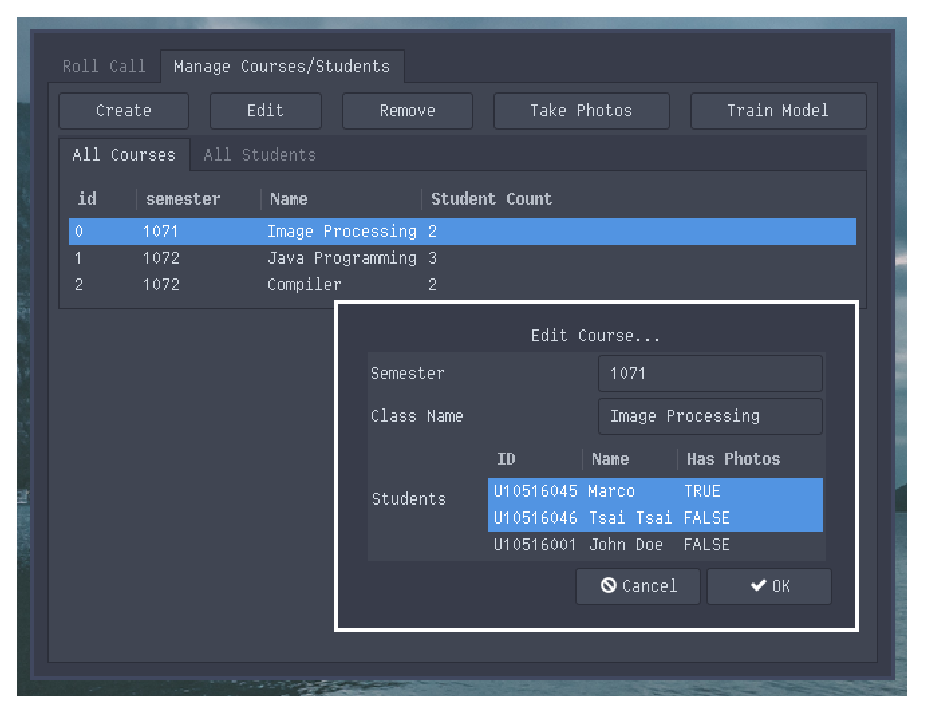
\includegraphics[width=\linewidth]{figures/preview1.eps}
    \caption{Managing courses.}
  \end{subfigure}
  \begin{subfigure}[b]{0.32\linewidth}
    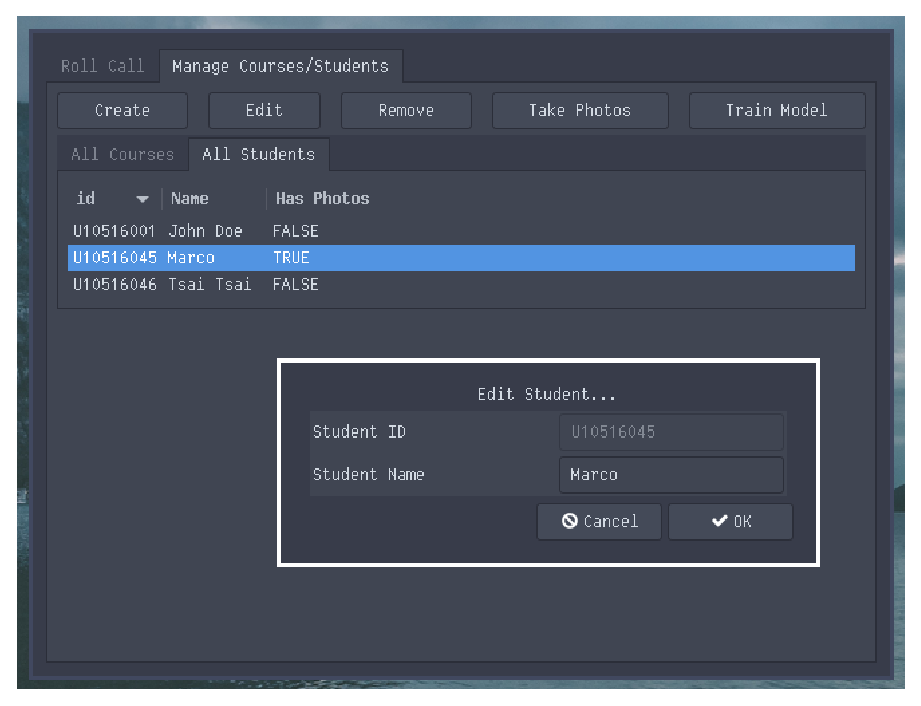
\includegraphics[width=\linewidth]{figures/preview2.eps}
    \caption{Managing students.}
  \end{subfigure}
  \begin{subfigure}[b]{0.32\linewidth}
    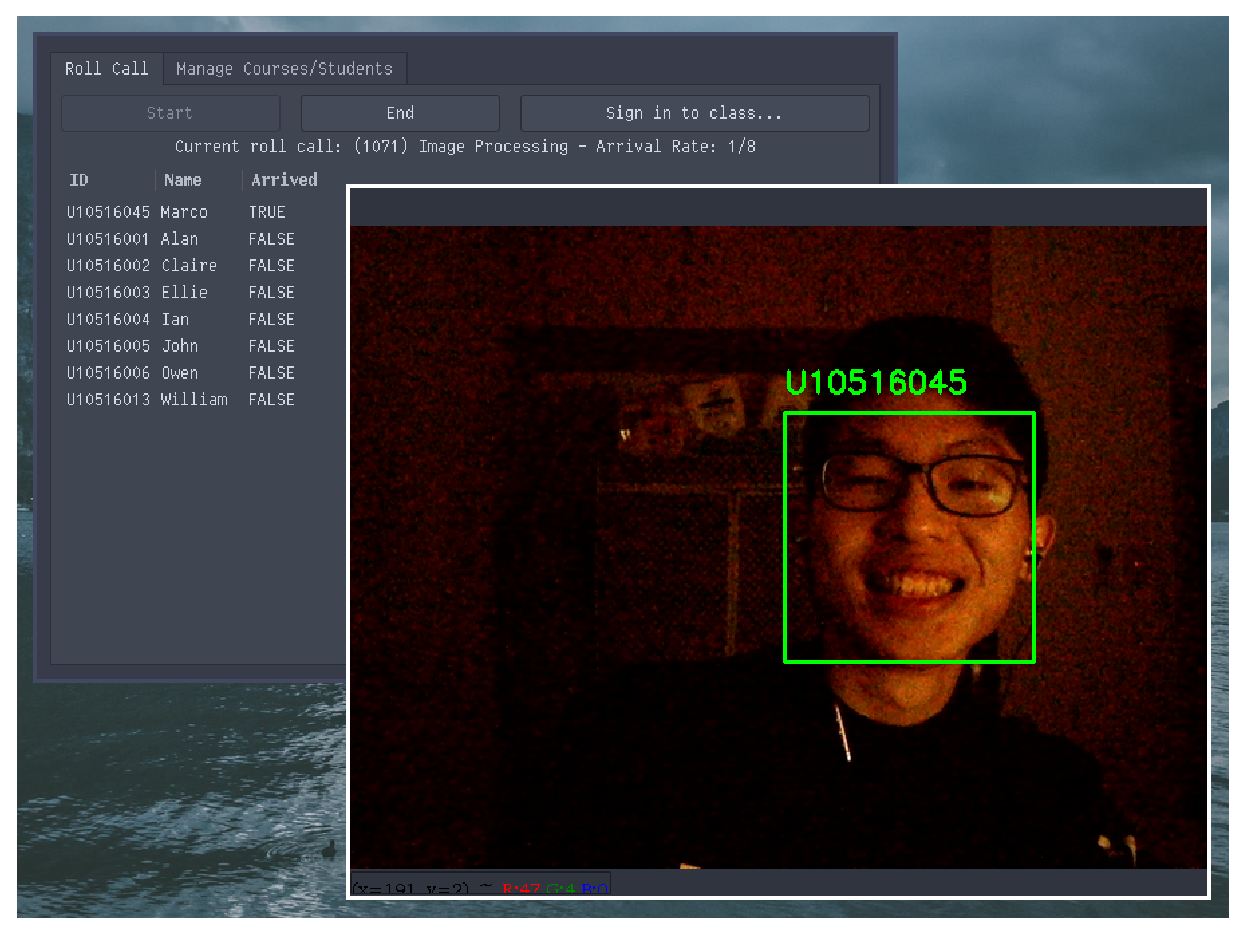
\includegraphics[width=\linewidth]{figures/preview3.eps}
    \caption{A student signing in.}
  \end{subfigure}
  \caption{PyRollCall running on a Linux machine with X11\protect\footnotemark \ installed.}
  \label{fig:systemAppearance}
\end{figure}
\vspace{0.5cm}

\footnotetext{X11, also known as X Window System, or simply X, is a windowing system that provides the basic framework for building GUI environments.}

%Another usage of this system is taking the photo of each student one by one as long as
%the size of the class is small enough. If the size of the class is too large, this apparently
%can result in longer waiting time for the students, and hence this approach is impractical.
%Consequently, our main objective is to ensure that the system can accurately recognize all the faces
%in a large image as possible as it can.

The actions available via PyRollCall's GUI are listed as follows:
\vspace{0.5cm}

\setstretch{0.8}
\begin{itemize}
  \item Maintain the data of the course and students they teach.
  \item Take photos of students with a camera and compute the facial embeddings.
  \item Perform roll calls.
  \item Export the results of roll calls to files.
\end{itemize}
\setstretch{\myContentLineSpacing}


\vspace{0.5cm}
Now that we have understood the prerequisites of the facial recognition features in PyRollCall,
it is time that we get to the installation details of this system. PyRollCall is able to run on Windows,
macOS and unix-like systems as long as the system supports Python 3 and GUI applications.
Furthermore, PyRollCall is open-sourced and managed with \emph{git}\footnote{git is a distributed
  version control system used for tracking file content changes in source code during software development},
and all of its external dependencies are already packaged in the project via Python's {virtualenv}\footnote{\
  virtualenv is a tool to created isolated Python environments by maintaining a set of libraries that a specific application depends on.},
thus the users do not have to worry about what and which versions of libraries they need to install. To checkout and run the project:

%Windows and macOS should natively support GUI applications. However, if you are running Linux,
%some distributions such as CentOS, Arch and Gentoo might not, by default, support
%GUI applications. In this case, you'll have to manually install X11 packages on your system.


\begin{lstlisting}[numbers=none,xleftmargin=0em,caption={Shell commands to checkout and run PyRollCall}]
$ git clone https://github.com/aesophor/pyrollcall.git
$ cd pyrollcall
$ source venv/bin/activate
$ ./pyrollcall.py 
\end{lstlisting}

The entry point to the system is \emph{pyrollcall.py}, a script located under the project's root directory.
Before running it, source the shell script \emph{venv/bin/activate} to activate the project's virtual environment.

\mySection{PyRollCall Libraries}

\subsection{OpenCV 4.1.1.26}
OpenCV (Open Source Computer Vision) is a cross-platform computer vision and machine learning library which was
originally developed by Intel Corporation. It can be used to develop real-time image processing, computer vision
as well as pattern recognition programs. The library is primarily written in C++, thus most interface of
OpenCV is for C++ and C. It also has bindings for other programming languages such as Python, Java and MATLAB.
Our project utilizes OpenCV for capturing images from a camera.

\subsection{dlib 19.18.0}
Dlib is a modern C++ toolkit containing machine learning algorithms and tools to solve complex real world problems.
It is widely used in various fields such as robotics, embedded devices, mobile phones, and large high performance
computing environments. The specific use of \emph{dlib} in PyRollCall is employing deep metric learning algorithms
and dlib models to solve facial recognition tasks.

\subsection{face\_recognition 1.2.3}
face\_recognition is an easy-to-use face recognition library which is built upon dlib's state-of-the-art
deep metric learning model with an accuracy of 99.38\%. We use face\_recognition to detect faces in an image,
estimate facial landmarks, compute a 128-d measurement for each face and perform facial classification.

\mySection{The Design of PyRollCall}
In this section, we present the use cases and the design of PyRollCall's architecture.
In the following context, a "user" refers to a "teacher" who wishes to perform roll calls
using PyRollCall, since the end user of this system is typically a teacher. In other words,
students are not the direct users of this system.
Figure~\ref{fig:use-case-diagram} shows the use case diagram of PyRollCall, whereas
Figure~\ref{fig:system-architecture} shows the system architecture of PyRollCall.


\subsection{Use Cases}
\vspace{0.5cm}

\setstretch{1.0}
\begin{itemize}
  \item Users can maintain the data of the courses and students they teach.
  \item Users can collect students' photos and generate their facial measurements.
  \item Users can start a roll call, recording students' attendace via FRT.
  \item Users can export the results of roll calls to files.
  \item Users should be able to keep their data the next time they use the system.
  \end{itemize}
\setstretch{\myContentLineSpacing}

\begin{figure}[!htb]
  \centering
  \vspace{1cm}
  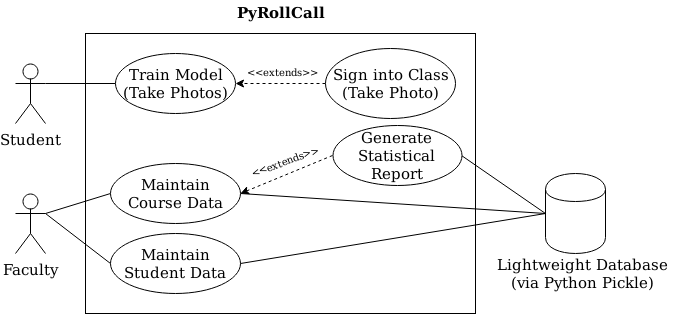
\includegraphics[width=\linewidth]{figures/use-case-diagram.png}
  \caption{Use Case Diagram}
  \label{fig:use-case-diagram}
  \vspace{1cm}
\end{figure}

\begin{figure}[!htb]
  \centering
  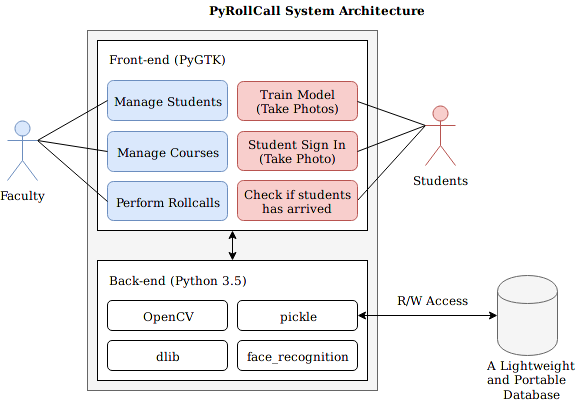
\includegraphics[width=\linewidth]{figures/system-architecture.png}
  \caption{System Architecture}
  \label{fig:system-architecture}
\end{figure}


\subsection{System Architecture}
The GUI is built with \emph{PyGTK}, giving users easy access to the
various functionalities in PyRollCall. Underneath the GUI, we use
\emph{OpenCV} to capture images via cameras, \emph{face\_recognition} and \emph{dlib} to
recognize faces of students, and \emph{pickle}\footnote{pickle is a Python module
  which implements binary protocols to serialize and deserialize Python objects.}
to serialize and deserialize facial measurements (or facial embeddings).
\vspace{0.5cm}

The user's data is saved in a lightweight database implemented by Python's pickle,
inclusive of the courses he or she teaches, the course-student mappings and
all the pre-computed facial embeddings of students.


\subsection{Implementation}
Text

\begin{algorithm}
\caption{A}
\label{alg:A}
\begin{algorithmic}
\STATE {set $r(t)=x(t)$}
\REPEAT
\STATE set $h(t)=r(t)$
\REPEAT
\STATE set $h(t)=r(t)$
\UNTIL{B}
\UNTIL{B}
\end{algorithmic}
\end{algorithm}


\myChapter{Experiments and Results}

\mySection{Experimental Settings}
In order to evaluate the accuracy of PyRollCall's facial recognition feature, we need at least two sets of photos.
The first set of photos, the \emph{training set}, is used to pre-compute facial embeddings.
The second set of photos, the \emph{testing set}, consists of the photos which have not appeared in the training set.
\vspace{0.5cm}

We randomly choose 20 celebrities as the participants of our experiments. For each individual, 30 photos
containing their faces are collected from the Internet and placed in the \emph{training set}, as shown in Figure~\ref{fig:training-set}.
Next, for each individual, we randomly collect an extra photo which is not in the training set, and place it in the \emph{testing set}.
Figure~\ref{fig:testing-set} shows one of the testing set used in our experiments.
\vspace{0.5cm}

In our experiments, we prepare one training set and three testing sets. Since the objective of our experiments is to test out
how accurate our system can handle the task of facial recognition under various circumstances,
we have three testing sets instead of one, which adds to the reliability of our experimental results.
Furthermore, we will assess how well the faces in the testing sets can be recognized with 5, 10, 15, 20, 25 and 30
facial embeddings pre-computed for each person, respectively.
\vspace{0.2cm}

\begin{figure}[!htb]
  \centering
  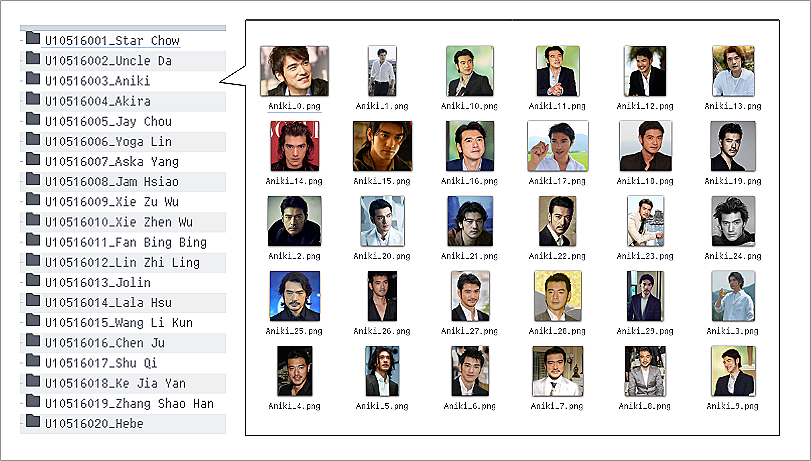
\includegraphics[width=\linewidth]{figures/training-set.png}
  \caption{The training set contains 30 photos per individual.}
  \label{fig:training-set}
\end{figure}
\vspace{0.5cm}

\begin{figure}[!htb]
  \centering
  \begin{subfigure}[b]{0.48\linewidth}
    
\includegraphics[width=\linewidth]{figures/testing-set.png}
    \caption{Before facial recognition.}
  \end{subfigure}
  \hfill
  \begin{subfigure}[b]{0.48\linewidth}
    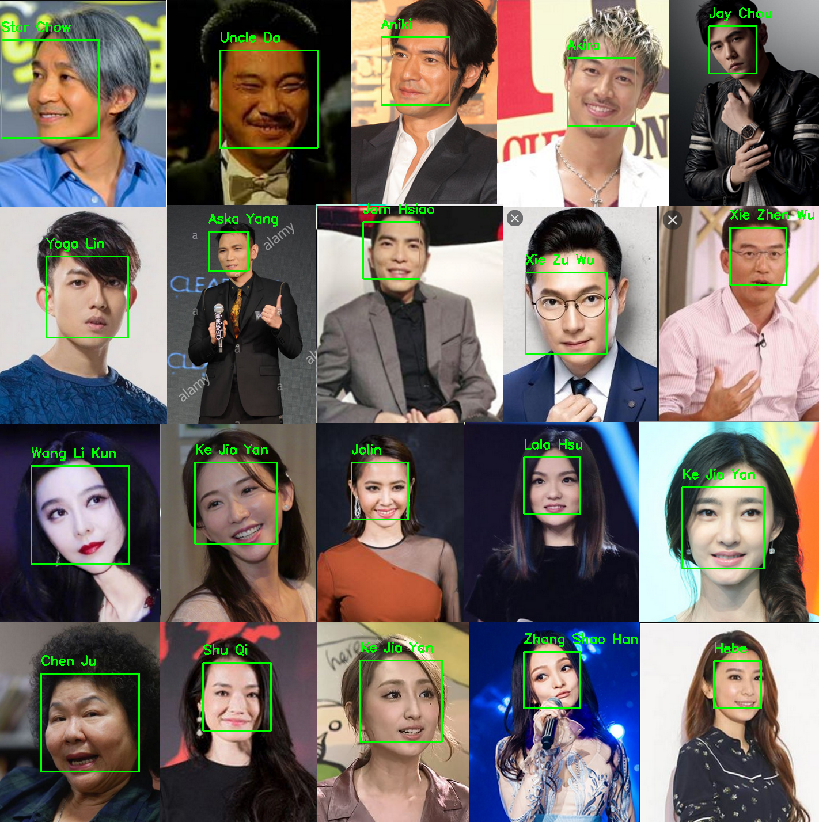
\includegraphics[width=\linewidth]{figures/testing-set-result.png}
    \caption{After facial recognition.}
  \end{subfigure}
  \caption{A testing set for assessing the accuracy of PyRollCall's facial recognition feature.}
  \label{fig:testing-set}
\end{figure}
\vspace{0.5cm}

\subsection{Experimental Result}
Text


\section{Conclusion and Future Research}
Text

\mySection{Conclusion}
In this thesis, we have proposed a roll call system using Deep Metric Learning and k-NN classification.
The system enables educational organizations to record students' attendance simply by taking a photo of
the entire classroom, thus saving a huge amount of time for both teachers and students.
we have also evaluated the practicality of our system by examining the accuracy of facial recognition.
\vspace{0.5cm}

Implemented in Python 3.5 and with the help of \emph{virtualenv}, PyRollCall is cross-platform and highly portable,
as all of its dependencies are already packaged with the project. It is implemented with \emph{OpenCV}
for capturing images from a camera, with \emph{face\_recognition} which is a wrapper library of \emph{dlib}
for performing facial recognition with Deep Metric Learning, and with \emph{PyGtk} for designing a user-friendly GUI.
\vspace{0.5cm}

There are two prerequisites of PyRollCall:

\begin{enumerate}
  \item The user should enter the data of all students and courses he or she teaches into the system; for each course, select the students that are currently taking it.
  \item Collect approximately 10 to 15 photos from each student and let the system pre-compute their facial embeddings (or encodings).
\end{enumerate}

\subsection{Future Research}
Text


\begin{thebibliography}{10}
  \addcontentsline{toc}{chapter}{Bibliography}

  \bibitem{latexcompanion} 
  Michel Goossens, Frank Mittelbach, and Alexander Samarin. 
  \textit{The \LaTeX\ Companion}. 
  Addison-Wesley, Reading, Massachusetts, 1993.

  \bibitem{einstein} 
  Albert Einstein. 
  \textit{Zur Elektrodynamik bewegter K{\"o}rper}. (German) 
  [\textit{On the electrodynamics of moving bodies}]. 
  Annalen der Physik, 322(10):891–921, 1905.

  \bibitem{knuthwebsite} 
  Knuth: Computers and Typesetting,
  \\\texttt{http://www-cs-faculty.stanford.edu/\~{}uno/abcde.html}

\end{thebibliography}


\end{document}
